\documentclass[runningheads]{llncs}

% Packages
\usepackage[T1]{fontenc}
\usepackage{graphicx}
\usepackage{amsmath}
\usepackage{booktabs}
\usepackage{placeins}
\usepackage{url}
\usepackage{orcidlink}

% ORCID helper
\renewcommand{\orcidID}[1]{%
  \nobreak\hspace{0.15em}\orcidlink{#1}%
}

\newcommand{\papertitle}{CATCH: Counterfactual Anatomical Tissue Inpainting with Conditional Haar-Wavelet Diffusion}
\hypersetup{
  hidelinks,
  pdftitle={CATCH: Counterfactual Anatomical Tissue Inpainting with Conditional Haar-Wavelet Diffusion},
  pdfauthor={Simon Winther Albertsen; Hjalte Bjoernstrup; Said Djafar Said; Mostafa Mehdipour Ghazi},
  pdfsubject={Conditional 3D diffusion for brain MRI inpainting},
  pdfkeywords={BraTS, brain MRI, inpainting, diffusion, Haar wavelets, trajectory aggregation}
}

% Figures path
\graphicspath{{figures/}}

% Paths for imported .tex files
\makeatletter
\def\input@path{{sections/}{tables/}}
\makeatother

\begin{document}

\title{\papertitle}
\titlerunning{CATCH: Conditional Haar-Wavelet Diffusion}

% Authors 
\author{
Simon Winther Albertsen\inst{1}\orcidID{0009-0004-0655-6664}
\and
Hjalte Bjoernstrup\inst{1}\orcidID{0009-0009-7757-4225}
\and
Said Djafar Said\inst{1}\orcidID{0009-0009-3570-2057}
\and
Mostafa Mehdipour Ghazi\inst{1,2}\orcidID{0000-0002-8473-281X}
}

% Running author
\authorrunning{S. W. Albertsen et al.}

% Institutes 
\institute{
Department of Computer Science, University of Copenhagen,
Copenhagen, Denmark\\
\email{\{zlp616,fhz806\}@alumni.ku.dk}
\and
Pioneer Centre for AI, Department of Computer Science,
University of Copenhagen, Copenhagen, Denmark\\
\email{ghazi@di.ku.dk}
}

\maketitle

% Content
% LEGACY, UNCOMPILED DRAFT FRAGMENT. The authoritative manuscript is ../main.tex.
\begin{abstract}
The BraTS local-synthesis task asks for plausible tumor-free tissue to be generated
inside a masked region of a T1-weighted brain MRI while preserving the observed
anatomy. We present CATCH, a conditional 3D diffusion framework operating on an
invertible Haar-wavelet representation. Its denoiser receives noisy target
subbands, voided-image subbands, and a signed mask. A tumor-excluded wavelet loss
with a hole-localized term provides supervision, while hard compositing preserves
every observed voxel. We compare fixed-mask training with strict random
tumor-component augmentation and a configured weighted mixture of tumor-derived,
blob, and ellipsoid masks. Arm-specific checkpoints and trajectory policies are
selected on development data, then frozen for a held-out 75-case confirmation
restricted to artificially removed healthy tissue. The selected weighted-mixture
pipeline (five trajectories, voxel-wise mean) achieved SSIM
$0.7972\pm0.1308$, PSNR $19.18\pm1.80$\,dB, and MSE
$0.009874\pm0.005359$ (mean $\pm$ sample SD). Against compute-matched random
augmentation, its mean improvements were $0.0188$ SSIM (95\% bootstrap CI:
$0.0127$--$0.0249$), $0.948$\,dB PSNR, and $0.002641$ MSE reduction; all three
corrected paired tests favored weighted mixture. Fixed-mask single-trajectory
inference achieved SSIM $0.7561\pm0.1615$. These within-CATCH results support the
complete weighted-mixture policy, but one training seed, arm-specific checkpoint
selection, and unequal trajectory counts relative to fixed mask limit causal and
cross-method conclusions.

\keywords{MRI inpainting \and Brain MRI \and Medical image synthesis
\and Diffusion models \and Wavelet transform \and BraTS}
\end{abstract}

% LEGACY, UNCOMPILED DRAFT FRAGMENT. The authoritative manuscript is ../main.tex.
\section{Introduction}
\label{sec:introduction}

Brain tumors alter local anatomy and violate the healthy-tissue assumptions of many
registration, parcellation, and atlas-based neuroimaging pipelines. Counterfactual
inpainting replaces a pathological region with plausible tumor-free tissue so that
such tools can operate on a completed image. The BraTS local-synthesis
task~\cite{kofler2023inpainting} formalizes this problem: given a voided T1n
(\emph{T1-weighted native}) volume and its inpainting mask, synthesize the missing
anatomy while leaving all observed voxels unchanged.

Diffusion models~\cite{ho2020ddpm} provide effective conditional
generators~\cite{lugmayr2022repaint,saharia2022palette}. Direct full-resolution 3D
diffusion is memory intensive, however. Wavelet diffusion models
(WDM)~\cite{friedrich2024wdm} reduce this cost through a fixed, invertible spatial
transform, and conditional WDM~\cite{friedrich2024cwdm} extends the formulation to
image-to-image tasks. We adapt it as CATCH (\textbf{C}ounterfactual
\textbf{A}natomical \textbf{T}issue Inpainting with \textbf{C}onditional
\textbf{H}aar-wavelet diffusion) and ask how healthy training holes should be
sampled.

Our contributions are:
\begin{itemize}
  \item conditional 3D Haar-wavelet diffusion with tumor-excluded supervision and
  voxel-exact preservation outside the requested hole;
  \item a within-CATCH comparison of fixed-mask, strict random, and
  weighted-mixture healthy-mask training variants, with compute-matched random
  versus weighted inference;
  \item development-only checkpoint and trajectory-policy selection followed by a
  frozen 75-case confirmation with paired uncertainty, patient-disjoint
  sensitivity, and audited examples.
\end{itemize}

% LEGACY, UNCOMPILED DRAFT FRAGMENT. The authoritative manuscript is ../main.tex.
\section{Related Work}
\label{sec:related-work}

\paragraph{Diffusion and inpainting.}
Denoising diffusion probabilistic models (DDPMs) learn the reverse of a gradual
noising process~\cite{ho2020ddpm}; score-based formulations connect this process to
stochastic differential equations~\cite{song2021scoresde}. RePaint conditions an
unconditional model by repeatedly restoring known pixels during
sampling~\cite{lugmayr2022repaint}, whereas Palette passes the observed image to a
conditional denoiser~\cite{saharia2022palette}. CATCH follows the latter approach
and enforces the known region once more by final hard compositing.

\paragraph{Volumetric medical synthesis.}
Learned latent spaces reduce high-resolution diffusion
cost~\cite{rombach2022ldm}; WDM instead uses an exactly invertible 3D wavelet
transform~\cite{friedrich2024wdm}. Its conditional extension supports volumetric
image-to-image synthesis~\cite{friedrich2024cwdm}. Diffusion has also been applied
directly to 3D healthy-brain inpainting~\cite{durrer2024inpainting} in the BraTS
local-synthesis setting~\cite{kofler2023inpainting}, whose data build on the wider
BraTS benchmark~\cite{menze2015brats,bakas2017advancing,baid2021rsna}. More
recently, fastWDM3D targets the substantial sampling cost of wavelet-space
healthy-tissue inpainting with a shortened reverse
process~\cite{durrer2026fastwdm3d}. Our work retains full ancestral sampling and
tailors mask representation, loss support, online hole sampling, and
development-selected trajectory aggregation; differing cohorts and protocols
preclude a direct score comparison.

\section{Method}
\label{sec:method}

CATCH adapts Tooth-Diffusion~\cite{said2025toothdiffusion} from dental CBCT
synthesis to brain-MRI inpainting.

Let $x_v$ be the voided T1n volume and
$m\in\{0,1\}^{H\times W\times D}$ the full region to inpaint. During training, the
provided mask is partitioned into an artificially removed healthy region $m_h$ and a
real tumor region $m_u$. The complete T1n volume $x$ supplies a target in $m_h$ but
still contains pathology in $m_u$, so the latter is excluded from supervision. Only
$x_v$ and $m$ are available to the model at inference.

\begin{figure}[!t]
  \centering
  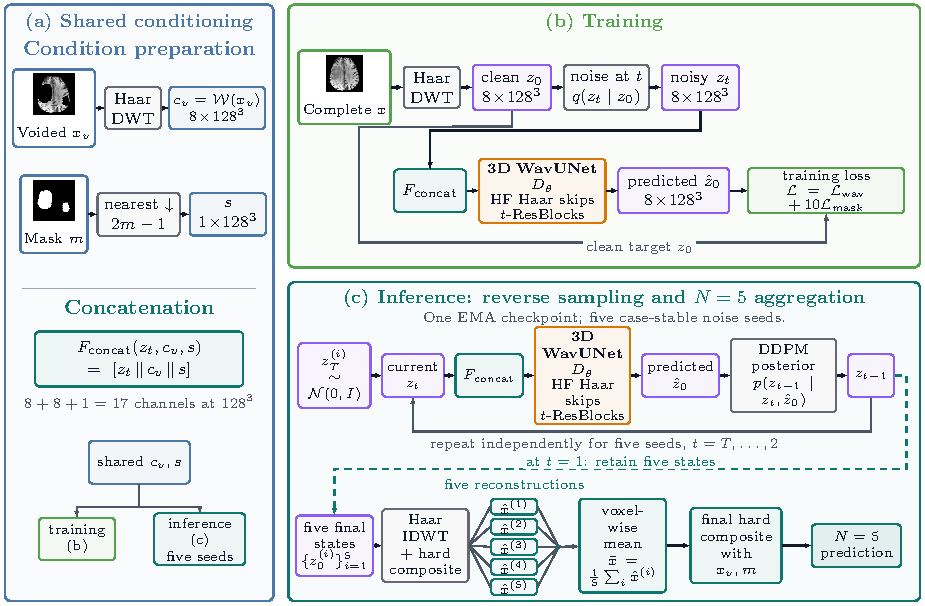
\includegraphics[width=0.98\textwidth]{catch_architecture}
  \caption{CATCH training and inference. A Haar transform maps the
  voided image to eight subbands, concatenated with noisy target subbands and a
  signed mask. WavUNet predicts clean coefficients; inverse transformation and hard
  compositing restore the observed region. For selected random and weighted models,
  five case-stable noise seeds traverse one EMA checkpoint; their reconstructions
  are averaged voxel-wise and composited again. Fixed mask uses $N=1$. Input
  thumbnails were selected without reconstruction metrics.}
  \label{fig:catch-architecture}
\end{figure}

\subsection{Conditional Wavelet Diffusion}
\label{sec:method:wavelet}

Volumes are reoriented to RAS and center-padded from
$240\times240\times155$ to $256^3$ without resampling. A one-level 3D Haar transform
$\mathcal W$ produces eight $128^3$ subbands; the LLL subband is divided by three
during modeling and restored before inversion, following WDM
\cite{friedrich2024wdm}. Thus the transform is fixed and invertible rather than a
learned autoencoder.

With $z_0=\mathcal W(x)$, the $T=1000$ forward process is
\begin{equation}
q(z_t\mid z_0)=\mathcal N\!\left(
z_t;\sqrt{\bar\alpha_t}z_0,(1-\bar\alpha_t)\mathbf I\right),
\end{equation}
using the variance-preserving SDE schedule~\cite{song2021scoresde} with
$\beta_{\min}=0.1$ and $\beta_{\max}=20$. The network predicts the clean
coefficients $\hat z_0$ directly and uses fixed-large reverse variance.

The voided image becomes $c_v=\mathcal W(x_v)$. We nearest-neighbor downsample $m$
to the wavelet grid and encode it as
$s=2\,\mathrm{NN}(m)-1\in\{-1,1\}^{128^3}$. The denoiser receives
\begin{equation}
\hat z_0=D_\theta([z_t\|c_v\|s],t),
\end{equation}
a 17-channel input. We call $D_\theta$ \emph{WavUNet}, a fully 3D wavelet U-Net
\cite{ronneberger2015unet,friedrich2024wdm} with base width 64, channel multipliers
$(1,2,2,4,4,4)$, two residual blocks per level, GroupNorm, SiLU, timestep
scale-and-shift modulation, wavelet skip connections, and no self-attention.

\subsection{Healthy-Tissue Objective}
\label{sec:method:objective}

The target and condition share the inference-available scale
$a=\max(x_v)$, are clipped to $[0,1]$, and mapped to $[-1,1]$. Let
$e_{k,p}=(\hat z_0^{(k)}(p)-z_0^{(k)}(p))^2$. A wavelet cell is assigned
$u_p=0$ if its corresponding $2^3$ voxel cell intersects $m_u$, and $u_p=1$
otherwise. The base loss is
\begin{equation}
\mathcal L_{\mathrm{wav}}=
\frac{1}{8|\Omega|}\sum_{k=1}^{8}\sum_{p\in\Omega}u_p e_{k,p}.
\end{equation}
For the hole-focused term, cells intersecting $m_h$ form a binary coverage map that
is Gaussian-smoothed ($\sigma=2$ on the wavelet grid) and multiplied by $u$ to
produce $w_p\ge0$. We use
\begin{equation}
\mathcal L_{\mathrm{mask}}=
\frac{\sum_{k,p}w_p e_{k,p}}{8\sum_p w_p},
\qquad
\mathcal L=\mathcal L_{\mathrm{wav}}+10\mathcal L_{\mathrm{mask}}.
\end{equation}
Normalizing by active mask mass keeps the regional coefficient comparable across
hole sizes. Both terms exclude cells touching the real tumor.

\subsection{Healthy-Mask Training Variants}
\label{sec:method:augmentation}

The \emph{fixed-mask} variant uses the supplied healthy mask. Online variants
sample $m_h'$, void $m_h'\cup m_u$, and supervise $m_h'$ while excluding $m_u$.
Their tumor-component bank contains only the 1,151 optimization cases, and each
variant has five repeat slots per case.

\emph{Random augmentation} is a strict reference-style policy: tumor components
only; current-case components allowed; inverse tumor-to-brain-ratio rank sampling
within a conditioned 10\% window; reference flips and rotations; five slots fixed
across epochs; and an error after exhausted placement.

\emph{Weighted-mixture augmentation} configures 80\% tumor components, 15\%
irregular blobs, and 5\% ellipsoids. It excludes current-case components, samples
empirical volumes, applies bounded 3D rotations and optional anisotropic scaling,
and refreshes slots by epoch. Generated masks are connected, contain
800--225,070 voxels, remain at least five voxels from $m_u$, and overlap background by at
most 25\%. Exhausted generation falls back to a supplied mask verified only as
nonempty and nonoverlapping with $m_u$.

\begin{figure}[!t]
  \centering
  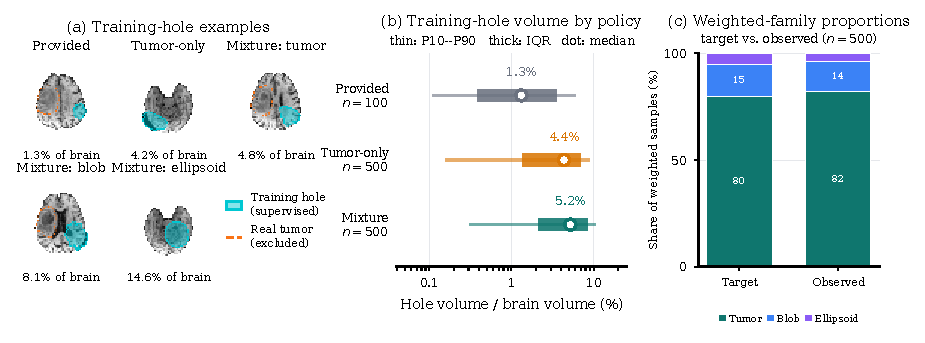
\includegraphics[width=\textwidth]{mask_augmentation_audit}
  \caption{Artificial training holes. (a) Fixed uses the supplied healthy mask,
  random uses tumor-derived masks only, and weighted mixture samples tumor, blob,
  or ellipsoid shapes. Cyan is the supervised hole; dashed orange is real tumor
  excluded from supervision. Percentages give 3D hole/brain volume. (b) Epoch-0
  size audit over 100 optimization cases (thin: 10th--90th percentiles; thick:
  interquartile range; circle: median; $n=100/500/500$; seed 0). Weighted realizes
  82.2/14.0/3.8\% tumor/blob/ellipsoid masks with no fallback. This describes the
  training distribution, not reconstruction quality.}
  \label{fig:mask-augmentation-audit}
\end{figure}

\subsection{Sampling and Compositing}
\label{sec:method:inference}

We use exponential-moving-average (EMA) weights and the complete 1000-step
ancestral reverse process. At each step, \texttt{clip\_denoised=True}
inverse-transforms the predicted clean state, clips it in normalized voxel space,
and transforms it back. The final reconstruction is restored to native intensity,
shape, and orientation, then hard-composited:
\begin{equation}
\hat x=x_v\odot(1-m)+\hat x_{\mathrm{gen}}\odot m,
\end{equation}
Global seed 0 and the case- and member-stable
\texttt{brats-validation-noise-v1} schema make trajectories shard-independent;
larger candidate sizes share the first $N$ seeds. Multi-trajectory policies decode
and composite each reconstruction, aggregate them voxel-wise by mean or median,
then composite again. This aggregates trajectories from one checkpoint, not
separately trained models.

% LEGACY, UNCOMPILED DRAFT FRAGMENT. The authoritative manuscript is ../main.tex.
\section{Experiments}
\label{sec:experiments}

\subsection{Data and Split Protocol}
\label{sec:exp:data}

The ASNR-MICCAI BraTS Local Synthesis release
\cite{kofler2023inpainting,menze2015brats,bakas2017advancing,baid2021rsna,akbari2017segmentation}
contains 1,251 training cases with complete and voided T1n, a full mask, and healthy
and unhealthy sub-masks. Organizer-validation ground truth is hidden.

A deterministic 100-case hold-out (seed 2026) leaves 1,151 optimization cases;
hold-out IDs are excluded from both the loader and component bank. Its checked-in
25-case development subset selects inference policy; the complementary 75-case
manifest is used by all confirmation pipelines. Development and confirmation
patients are disjoint, but the split is case-keyed: 3/25 development and 11/75
confirmation cases have an optimization-pool sibling timepoint. The five diagnostic
cases have none. We add a post-hoc sensitivity analysis on the 64 confirmation
cases patient-disjoint from optimization.

\subsection{Training and Checkpoint Selection}
\label{sec:exp:training}

We compare three max-normalized, 17-channel concatenation training variants with
fixed-mask, random-augmentation, or weighted-mixture healthy-mask policies. Each
uses training seed 0, batch size one per GPU,
AdamW~\cite{loshchilov2019adamw} with learning rate $10^{-5}$ and zero weight decay,
a 300,000-step linear-decay horizon, and EMA decay 0.9999. Training is FP32 on
NVIDIA A100 40\,GB GPUs; checkpoints are saved every 5,000 steps.

Every 10,000 steps, EMA diagnostics use one deterministic full 1000-step DDPM
trajectory on five development cases (fixed-mask 200,000 is absent). Within each
variant, recorded checkpoints are ranked by aggregate structural similarity index
measure (SSIM, descending), peak signal-to-noise ratio (PSNR, descending), and mean
squared error (MSE, ascending), then by their mean rank. Fixed-mask 170,000 and
180,000 tie; we retain 180,000 because it leads PSNR and MSE. Random 290,000 and
weighted-mixture 200,000 uniquely minimize joint rank. These diagnostics select
checkpoints, not final performance.

\subsection{Inference Selection and Evaluation}
\label{sec:exp:selection}

At each terminal EMA checkpoint (step 299,999), the 25 development cases compare
nested $N\in\{1,3,5\}$ trajectories with voxel-wise mean or median aggregation.
Global seed 0 and \texttt{brats-validation-noise-v1} give stable case and member seeds
and shared first members across $N$. Mean $N=5$ is selected for random and weighted
mixture. For fixed mask, mean $N=3$ lowers joint rank from 2.9200 to 2.7867 at
three times the trajectories, while mean $N=5$ is worse (3.2400); we retain $N=1$.
Policies transfer unchanged to selected checkpoints and are frozen before
confirmation.

The official evaluator normalizes prediction and target to $[0,1]$ from the
voided-image 0.5th and 99.5th percentiles and scores only the provided healthy mask.
We report SSIM and PSNR (higher is better), MSE (lower is better), and their mean
within-case rank among selected pipelines. Means and sample SDs describe 75-case
heterogeneity, not training-seed variability. Per metric, a Friedman test precedes
two-sided paired Wilcoxon tests, Holm-adjusted over three contrasts. Mean paired
improvements use deterministic 100,000-resample case-bootstrap 95\% intervals
(seed 2026). Compressed NIfTI predictions, per-case metrics, split audits, hashes,
and metadata are retained as CSV/JSON. Code, paper artifacts, and analysis scripts
will be released at
\url{https://github.com/simonwinther/brats2026}.

% sections/05_results.tex

\section{Results}
\label{sec:results}

The final seed-0 training runs and locked confirmation evaluations were still in
progress when this manuscript revision was prepared. We therefore do not promote the
five-case monitoring curves to quantitative results. Those curves are intended for
training diagnostics only and are especially unsuitable for comparison with earlier
runs, which used a different mask-loss normalization and a different five-case
monitoring cohort.

To make the development history auditable while the final evaluations are pending,
Fig.~\ref{fig:training-dynamics} records four corrected-run histories, including the
exploratory FiLM branch. The figure uses raw validation events without dashboard
smoothing and is a training diagnostic rather than evidence for the final method
ranking.

\begin{figure}[t]
  \centering
  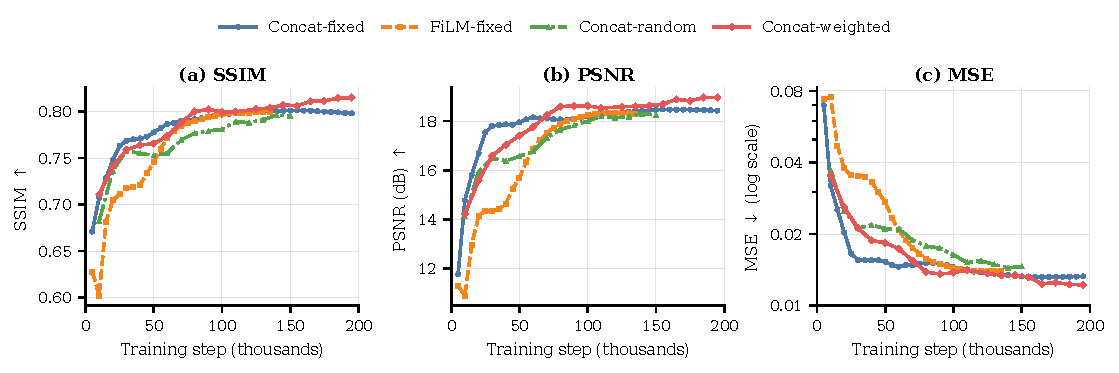
\includegraphics[width=\textwidth]{training_dynamics}
  \caption{Interim EMA diagnostics for four seed-0 development runs on the same
  deterministic five-case monitoring cohort. The snapshot contains concat fixed,
  concat random, concat weighted, and exploratory FiLM weighted runs. Fixed-mask
  monitoring occurs every 5,000 steps and augmented-run monitoring every 10,000
  steps. Curves end at the latest available event and are not used for checkpoint or
  method selection. Final claims use the predeclared development and confirmation
  cohorts.}
  \label{fig:training-dynamics}
\end{figure}

The incomplete intermediate-checkpoint screen is not used for model selection or
reported as a final result. Ensemble selection uses saved per-case metrics on the
fixed 25-case development subset without dashboard smoothing.

\subsection{Development-Set Ensemble Selection}
\label{sec:results:ensemble-selection}
% Canonical per-case sources on Hendrix:
% results/paper300k-concat-fixed-s0-maxnorm-dev25-ensemble-screen-n5/ensemble_metrics/
% results/paper300k-concat-random-s0-maxnorm-dev25-ensemble-screen-n5/ensemble_metrics/
% results/paper300k-concat-weighted-s0-maxnorm-dev25-ensemble-screen-n5/ensemble_metrics/

Table~\ref{tab:ensemble-selection} reports the preconfirmation ensemble screen on
the 25-case development subset. For the fixed-mask arm, ensembling had no material
effect on the aggregate metrics: over all five candidates, SSIM spanned only
$0.709715$--$0.709722$, PSNR $18.178827$--$18.179194$ dB, and MSE
$0.015027$--$0.015028$ at the reported precision. Although distinct seeds changed
the reconstruction inside the scored healthy region for all 25 cases, averaging did
not consistently reduce the fixed arm's error.

The random and weighted augmentation arms behaved differently. Mean aggregation
with $N=5$ achieved the lowest joint rank for both arms, whereas $N=1$ ranked last.
The fixed arm slightly preferred mean aggregation with $N=3$ by rank, but its
aggregate metric differences were negligible and mean $N=5$ was worse than $N=1$.
Given that five trajectories require approximately five times as many sampler calls,
we freeze $N=1$ for the fixed arm and mean $N=5$ for the random and weighted arms.
The random and weighted runs also retain their first-trajectory $N=1$ outputs, so the
confirmation results can distinguish an equal-sampling comparison from the selected
arm-specific inference policies.

\begin{table}[b]
  \centering
  \caption{Challenge-style mean rank on the 25-case development subset for the
  terminal EMA checkpoints. Ranks are averaged over SSIM, PSNR, and MSE; lower is
  better. The $N=1$ mean/median duplicate is shown once. Bold values mark the best
  configuration within each column.}
  \label{tab:ensemble-selection}
  \small
  \setlength{\tabcolsep}{5pt}
  \begin{tabular}{@{}lrrrr@{}}
    \toprule
    Configuration & Fixed & Random & Weighted & Pooled \\
    \midrule
    $N=1$                 & 2.9200 & 4.7067 & 4.4000 & 4.0089 \\
    Mean, $N=3$           & \textbf{2.7867} & 2.1333 & 2.6933 & 2.5378 \\
    Median, $N=3$         & 2.9733 & 3.5333 & 3.7733 & 3.4267 \\
    Mean, $N=5$           & 3.2400 & \textbf{1.6000} & \textbf{1.5867}
                          & \textbf{2.1422} \\
    Median, $N=5$         & 3.0800 & 3.0267 & 2.5467 & 2.8844 \\
    \bottomrule
  \end{tabular}
\end{table}

% Activate these templates after the corresponding manifests have been audited.
% The checkpoint and ensemble figures should replace the interim training-dynamics
% figure if space is limited.
%
% \begin{figure}[t]
%   \centering
%   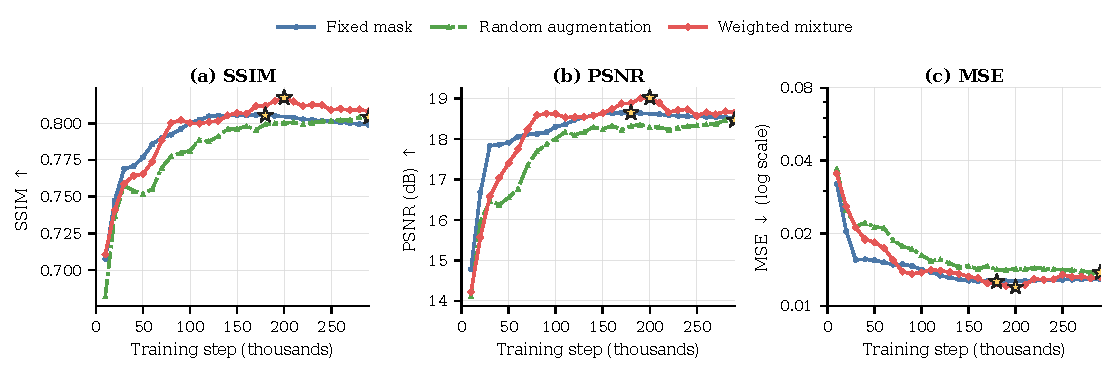
\includegraphics[width=\textwidth]{checkpoint_selection}
%   \caption{Checkpoint selection on the fixed 25-case development subset. Panels
%   show the candidate means for SSIM, PSNR, and MSE and the paired joint rank
%   obtained by averaging per-case ranks across the three challenge metrics. The
%   star marks the lowest-rank candidate. No dashboard smoothing is applied.}
%   \label{fig:checkpoint-selection}
% \end{figure}
%
% \begin{figure}[t]
%   \centering
%   \includegraphics[width=\textwidth]{ensemble_selection}
%   \caption{Ensemble selection on the same 25 development cases. Mean and median
%   aggregation are compared for one, three, and five seeded reconstructions per
%   case using the checkpoint-selection rank rule.}
%   \label{fig:ensemble-selection}
% \end{figure}

The final quantitative table will be populated from the immutable aggregate JSON and
per-case CSV files produced by the shared evaluator. Its primary columns will report
mean $\pm$ sample standard deviation for SSIM, PSNR, and MSE on the locked 75-case
confirmation cohort. Autoencoder and Pix2Pix baselines will be scored on the same
case manifests with the same official evaluator. The official validation submission
will be reported separately because its ground truth is hidden.

The qualitative figure will select the cases nearest the 10th, 50th, and 90th
percentiles of confirmation-cohort SSIM under the frozen method. Each row will show
the voided input, one-sample reconstruction, selected-ensemble reconstruction,
ground truth, and absolute-error maps. Case selection, slice selection, intensity
windows, and metric labels are deterministic and saved with the figure manifest.

% \begin{figure}[t]
%   \centering
%   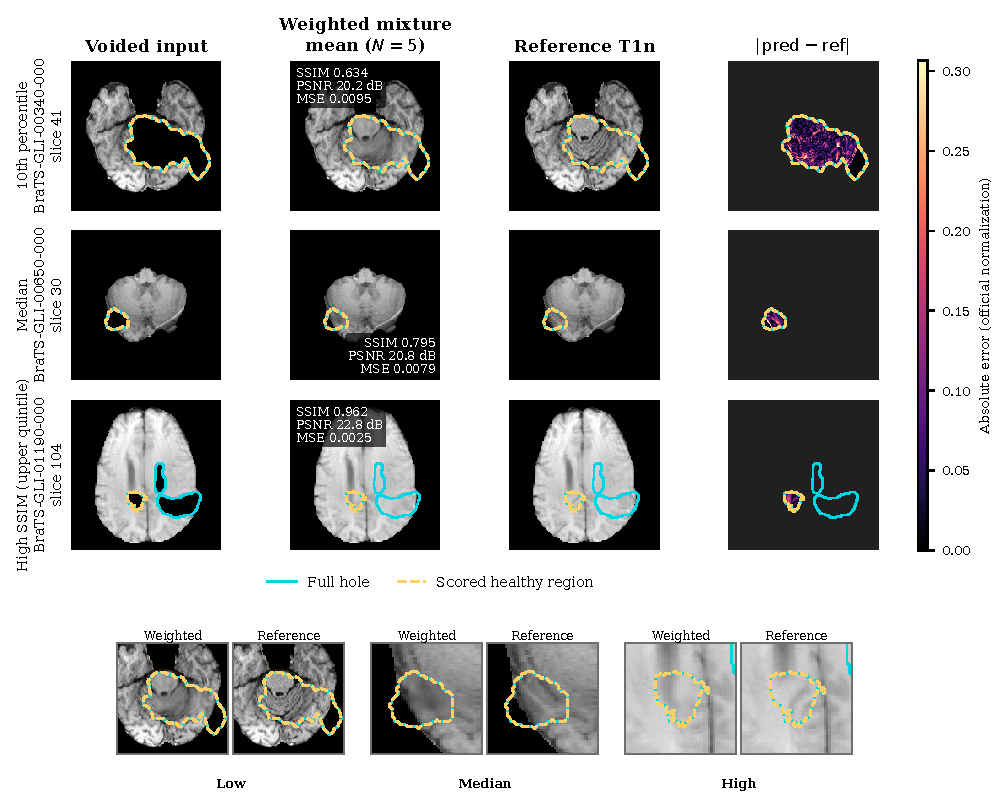
\includegraphics[width=\textwidth]{qualitative_reconstructions}
%   \caption{Representative reconstructions from the locked confirmation cohort.
%   Rows are selected deterministically at the 10th, 50th, and 90th percentiles of
%   frozen-method SSIM. Cyan outlines the complete inpainting hole and dashed yellow
%   outlines the healthy region used for scoring. All anatomical panels in a row use
%   one intensity window; both error columns use one pooled, 99th-percentile-clipped
%   normalized color scale.}
%   \label{fig:qualitative-reconstructions}
% \end{figure}

% TODO: Insert final figures and tables only after their manifests verify the
% predeclared case files, full-DDPM sampling, EMA weights, and frozen selection.

\FloatBarrier
\section{Discussion}
\label{sec:discussion}

Weighted mixture gives the strongest selected pipeline on held-out data. Random and
weighted use the same architecture, training horizon, mean-$N=5$ inference, split,
seeds, and evaluator; their contrast therefore matches inference compute. Their
training policies differ jointly in source families, size sampling, transforms,
whether current-case sources are eligible, epoch refresh, and fallback. Evidence
supports the full policy, not its configured 80/15/5 proportions alone. Gains in
most paired cases argue against an outlier-only effect, but 15 all-metric losses show
it is not uniformly superior. One training seed and arm-specific checkpoints
prevent component-level causal attribution.

The fixed-mask pipeline uses $N=1$ by design. On development data, mean $N=3$
improved joint rank by only 0.1333 at three times the trajectory count, while mean
$N=5$ was worse. Thus fixed versus augmented compares unequal trajectory counts;
weighted versus random is the equal-trajectory contrast.

The invertible wavelet representation enables full-volume 3D sampling, while hard
compositing preserves observed tissue. Sampling remains costly: mean $N=5$ runs
five 1000-step ancestral trajectories. Recent work on faster wavelet
inpainting~\cite{durrer2026fastwdm3d} motivates sampler validation under the same
frozen cohort and scoring protocol.

Metrics cover artificially removed healthy voxels. Because observed T1n remains
pathological in $m_u$, neither the metrics nor the qualitative reference establish
patient-specific counterfactual correctness there; such ground truth does not
exist. Plausible reconstructions may hallucinate incorrect anatomy and are not
clinically validated. Hidden organizer-validation ground truth prevents local
external scoring.

The case-keyed split is not fully patient-independent: optimization includes sibling
timepoints for 3/25 development and 11/75 confirmation cases; development and
confirmation patients are mutually disjoint. In a post-hoc 64-case patient-disjoint
analysis, weighted mixture obtains SSIM 0.8101, PSNR 19.27\,dB, and MSE 0.009220;
random obtains 0.7911, 18.33\,dB, and 0.011664; and fixed obtains 0.7703,
17.93\,dB, and 0.012764. The ordering is unchanged. This removes confirmation
overlap only, not possible influence on development-stage selection.

Other limitations are one seed per variant, five-case one-trajectory checkpoint
diagnostics, transfer of terminally selected inference policies to arm-specific
checkpoints, and no completed external baseline. Across-case variability does not
measure seed variability, so prior-method superiority is unestablished. Development
ranks lack their original per-case predictions; one random-arm dirty-worktree diff
was not preserved, although its checkpoint, configuration, metrics, sampling
metadata, and prediction hashes are archived. Future work should add seeds and
baselines, preserve all outputs, validate faster sampling, and use patient-level
splits and multimodal conditioning.

\section{Conclusion}
\label{sec:conclusion}

CATCH combines conditional 3D Haar-wavelet diffusion, tumor-excluded supervision,
hard preservation of observed tissue, and development-selected trajectory
aggregation. In this single-seed internal study, weighted-mixture augmentation is
strongest under matched compute on artificially removed healthy tissue; clinical
and cross-method superiority remain unestablished.

% LEGACY, UNCOMPILED DRAFT FRAGMENT. The authoritative manuscript is ../main.tex.
\begin{credits}
\subsubsection{\ackname}
We thank the University of Copenhagen and Pioneer Centre for AI. Compute used
Hendrix; Challenge data came through Synapse ID syn74274097.

\subsubsection{\discintname}
The authors declare no competing interests.
\end{credits}


% Bibliography
\bibliographystyle{splncs04}
\bibliography{references}

\end{document}
